\localauthor{Johannes Garstenauer}

Im Folgenden soll die Qualität der Testsuites bestimmt werden,
um ihre Aussagekraft hinsichtlich der Bestätigung der Qualität des LaSes\-System zu evaluieren.
Hierzu wird die Quelltextüberdeckung der \emph{Unittests} sowie der \emph{Integrationstests} untersucht.
Schlußendlich werden die Ergebnisse interpretiert.

\subsection{Quelltextüberdeckung}\label{subsec:quelltextueberdeckung}
Zur Messung der Quelltextüberdeckung wurde die populäre \emph{Java Code Coverage Library \textbf{JaCoCo}} verwendet.
In der Analyse wird ein besonderes Augenmerk auf die Werte der \emph{Zeilen-} und \emph{Zweigüberdeckung} gelegt,
da diese am aussagekräftigsten bezüglich der Testqualität sind.

\subsubsection{Unit Tests}
Es existieren \emph{Whiteboxtests} zu den meisten Klassen und Methoden des Projekts.
Es besteht jedoch kein Anspruch auf Vollständigkeit.
Die \emph{Unittests} entstanden größtenteils parallel zur Entwicklung.
Bestimmte Arten von Klassen wurden hierbei ausgespart:

\begin{itemize}
    \item \emph{Backing-Beans}: Es bestand die Erwartung, dass diese sinnvoller in den \emph{Blackboxtests}
    abgedeckt werden können.
    \item \emph{Klassen in den internal-Paketen}: Hier war in der Regel ein großer \emph{Mockingaufwand} vonnöten,
    um erwartetes Verhalten testen zu können.
    Dies liegt an der großen Anzahl von \emph{Jakarta Server Faces} spezifischen Komponenten,
    welche in diesen Klassen verwendet werden.
    Aufgrund des Wunsches, vonseiten der Entwickler, die begrenzte Entwicklungszeit
    wirkungsvoll einzusetzen und der oft überschaubaren \emph{JSF} fremden Logik, welche zu überprüfen war,
    wurden diese Klassen beim \emph{unittesting} oft ausgespart.
    Beispiele hierfür sind z.B. der \emph{UncheckedExceptionHandler} oder \emph{MessageResourceBundleProducer}.
\end{itemize}
Die \emph{Quelltextüberdeckungswerte} sind vor diesem Hintergrund zu betrachten.

\begin{figure}[h]
    \centering
    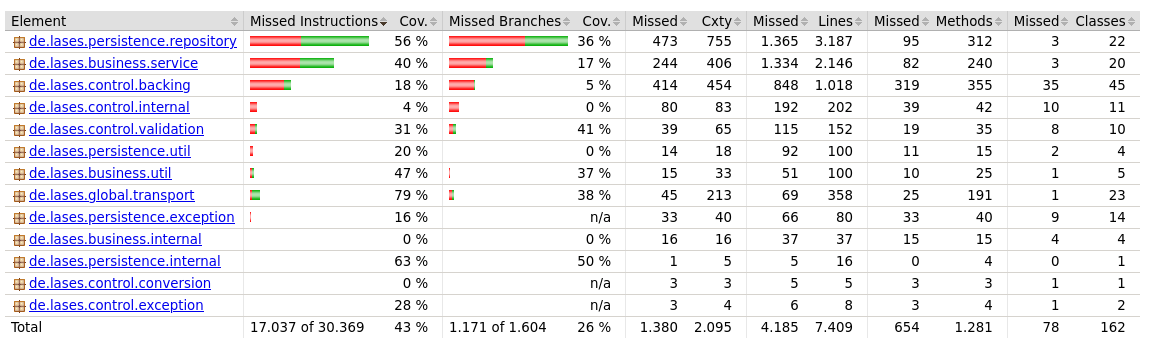
\includegraphics[width=0.9\linewidth]{graphics/coverage_unit}
    \caption{Übersicht über die genauen Überdeckungswerte (gegliedert nach Paketen)}
    \label{fig:coverage_unit}
\end{figure}

Die 96 Testmethoden der Unittests erreichen eine \emph{Zeilenüberdeckung} von \textbf{43\%}
und eine \emph{Zweigüberdeckung} von \textbf{26\%}.


\subsubsection{Integration Tests}
Die \emph{Blackboxtests} decken große Teile der vorgesehenen Funktionalität ab und beinhalten zusätzlich Tests
zu sicherheitskritischen Szenarien, wie \emph{Skript- und Sequelinjektionen}.
Es besteht wiederum kein Anspruch auf Vollständigkeit.
Erwartete Schwachstellen der \emph{Quelltextberdeckung} sind zu erwarten aufgrund von:
\begin{itemize}
    \item Den entgegengesetzten Prinzipien von \emph{Isolation} und \emph{Integration} im Software Testing.
    Integrationstests weisen eine höhere Integration (d.h. ein höheres Clustering der Features in den Tests)
    auf Kosten der Isolation auf und erreichen aufgrunddessen weniger Granularität, beispielsweise in der Zweigabdeckung.
    Daraus resultiert eine geringere \emph{Quelltextüberdeckung}.
    \item Codeabschnitte, welche sich der defensiven Programmierung widmen, werden seltener überdeckt
\end{itemize}
Die \emph{Quelltextüberdeckungswerte} sind vor diesem Hintergrund zu betrachten.

Die Integrationtests erreichen eine \emph{Zeilenüberdeckung} von \textbf{45\%}
und eine \emph{Zweigüberdeckung} von \textbf{34\%}.

\begin{figure}[h]
    \centering
    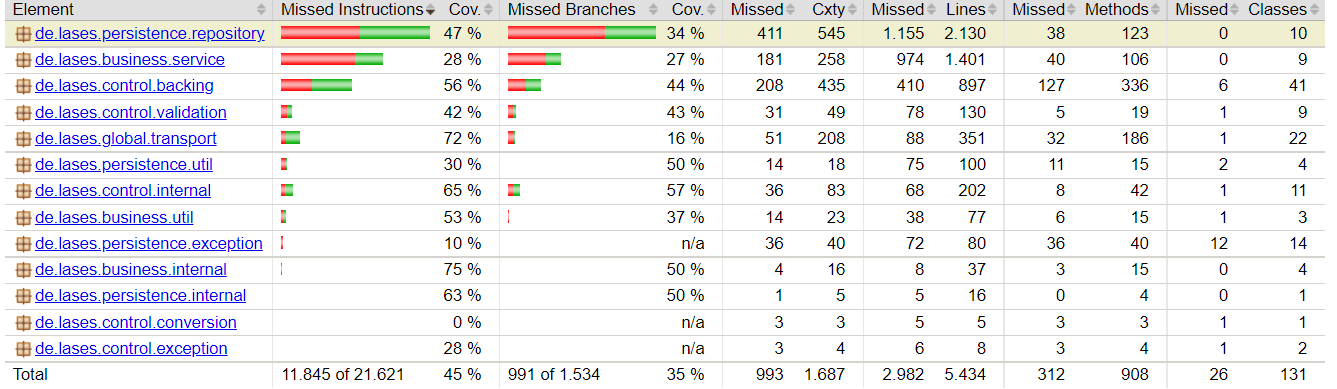
\includegraphics[width=0.9\linewidth]{graphics/coverage_it}
    \caption{Übersicht über die genauen Überdeckungswerte (gegliedert nach Paketen)}
    \label{fig:coverag_it}
\end{figure}